\documentclass{../mnblab}
\usepackage{pdfpages}

\titleinfo{
    title       = mnblab の学位論文フォーマット,
    title_en    = Formatting for mnblab theses,
    degree      = master,
    id          = 24MM016,
    author      = 金川 竜大,
    advisor     = 間邊 哲也 助教,
    year        = 2024,
    month       = 01,
    day         = 10,
}


\begin{document}
\maketitle
\begin{abstract}
	概要環境。この概要環境を使うことで、目次も出力され、ページ番号もローマ数字で本文と別になる。
\end{abstract}
\pagestyle{mnblab_main}

\chapter{ここは章}
\section{これが節}
\subsection{これは小節}
\subsubsection{ここまでも目次に乗る}
サンプルな文字
\newpage
\section{第2節めが}
\chapter{ぱーと2}
\chapter{第3章}
\chapter*{謝辞}
\begin{thebibliography}{99}
    \bibitem{生活時間@塩津} \href{https://doi.org/10.3130/aija.63.45_4}{塩津弥佳, 吉澤晋, 池田耕一, 野崎淳夫, ``生活時間調査による屋内滞在時間量と活動量 : 室内空気汚染物質に対する曝露量評価に関する基礎的研究 その1,'' 日本建築学会計画系論文集, vol.63, no.511, pp.45-52, Sept. 1998. DOI: 10.3130/aija.63.45\_4}
    \bibitem{GNSSの精度@児島} \href{https://doi.org/10.11485/itetr.34.6.0_153}{児島 伴幸, 柳澤 政生, 大附 辰夫, 戸川 望, ``歩行者の現在地認識に基づく道路標識とランドマークを用いた位置特定システムの改良とシミュレーション評価(ITS画像処理,映像メディア,視覚および一般),'' 映像情報メディア学会技術報告, vol.34.6, pp.153-158, 2010. DOI: 10.11485/itetr.34.6.0\_153}
    \bibitem{Proximity@Krumm} \href{https://doi.org/10.1007/978-3-540-30119-6_17}{J.~Krumm and K.~Hinckley, ``The NearMe Wireless Proximity Server,'' UbiComp 2004: Ubiquitous Computing, Nottingharm, UK, pp.283-300, Sept. 2004. DOI: 10.1007/978-3-540-30119-6\_17}
    \bibitem{Fingerprint@河口} \href{https://doi.org/10.1541/ieejeiss.126.1212}{伊藤 誠悟, 河口 信夫, ``アクセスポイントの選択を考慮したベイズ推定による無線LANハイブリット位置推定手法とその応用,'' 電気学会論文誌C(電子・情報・システム部門誌),'' vol.126, no.10, pp.1212-1220, Oct. 2006. DOI:10.1541/ieejeiss.126.1212}
    \bibitem{Fingerprint@Jie} \href{https://doi.org/10.1109/PERCOM.2005.7}{J.~Yin, Q.~Yang, and L.~Ni, ``Adaptive Temporal Radio Maps for Indoor Location Estimation,'' Third IEEE International Conference on Pervasive Computing and Communications, pp.85-94, March. 2005. DOI: 10.1109/PERCOM.2005.7}
    \bibitem{Lateration@Bahl} \href{https://doi.org/10.1109/INFCOM.2000.832252}{P.~Bahl and V.N.~Padmanabhan, ``RADAR: an in-building RF-based user location and tracking system,'' Proceedings IEEE INFOCOM 2000. Conference on Computer Communications. Nineteenth Annual Joint Conference of the IEEE Computer and Communications Societies (Cat. No.00CH37064), vol.2, pp.775-784, March. 2000. DOI: 10.1109/INFCOM.2000.832252}
\end{thebibliography}


\appendix

\chapter{附録一つ目}
\chapter{本研究に関する業績}

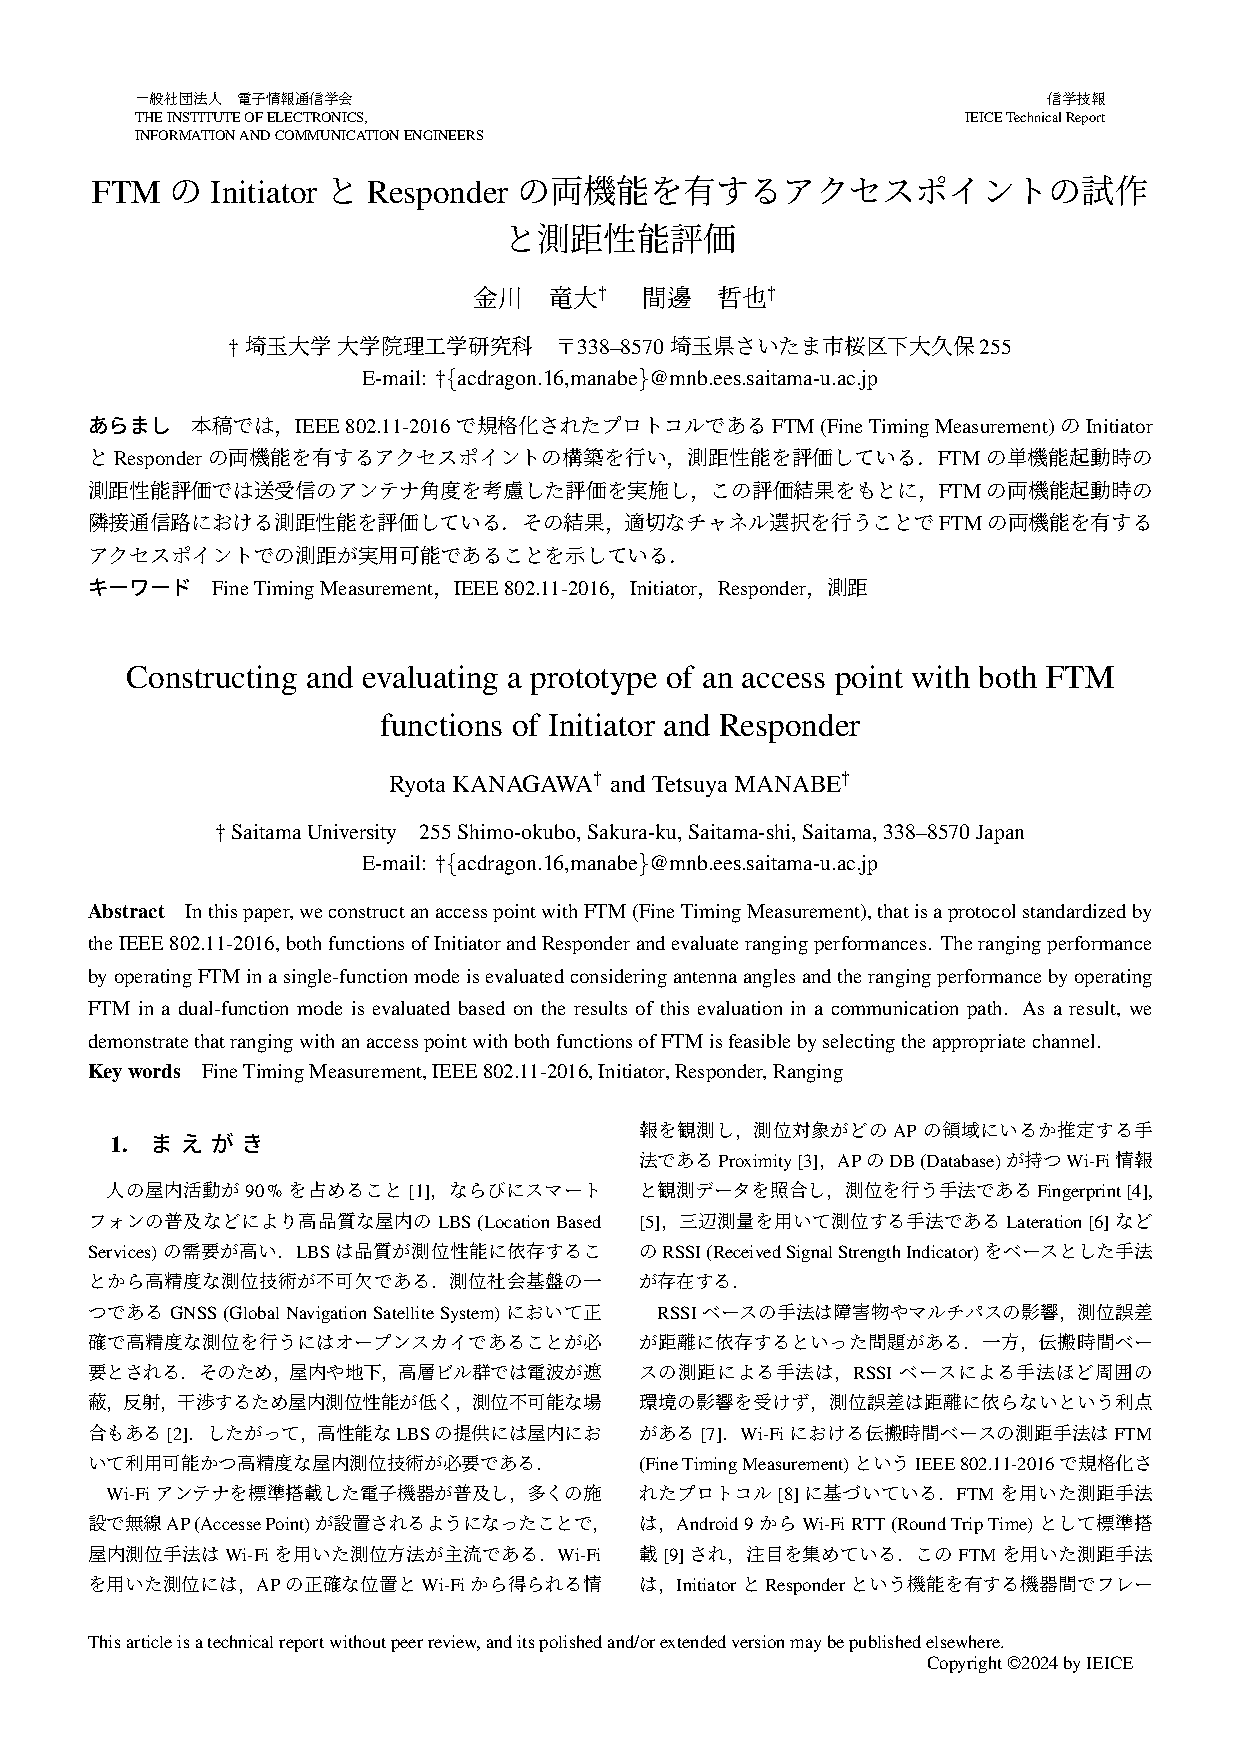
\includepdf[pages=-, pagecommand={\thispagestyle{empty}}, fitpaper]{../pdf/241205_ITS研究会@鹿児島_金川竜大.pdf}

\end{document}
